\chapter{Jim Rohn -- GSI Master Trainer Seminar 2003}

This chapter follows a Jim Rohn seminar talk in the order in which the argument is actually built. The lecture begins with a concrete economic puzzle, turns that puzzle into a ladder of arithmetic possibility, then repeatedly asks what inner change would make such an ascent real rather than merely imaginable. We will keep the numbers, the examples, and the transitions close to the spoken lecture, while writing them in a more deliberate note form.

\begin{remark}
These notes follow a Jim Rohn original talk from a curated playlist rather than a formal institutional course. The transcript is the primary source, and the present chapter is organized through the Video2Book workflow associated with LazyingArt LLC. No validated board screenshots survive for this lecture, so every displayed formula and diagram below is a cautious transcript-derived reconstruction rather than a transcription of visible board work.
\end{remark}

\section{Economic Philosophies and the Turn to Performance}

Rohn opens with a low-wage case and asks how such a situation is to be changed. He does not begin by praising ambition in general. Instead, he runs through a short menu of economic philosophies and lets us see, one by one, what each philosophy can and cannot do.

The first philosophy is to wait for public policy to change the minimum wage. The second is to wait for the company to move us from one hourly rate to a higher one. The third is to demand more money, especially as part of a group. The lecture is careful here: demand is not presented as nonsense. It can sometimes move the number. But it remains, in his vocabulary, a risky and limited strategy.

At the start of this sequence, the stable numerical objects are modest:
\begin{equation}
w_0=\$5/\text{hour}, \qquad w_1=\$6/\text{hour}.
\end{equation}
The point of the opening is not yet to produce wealth, but to ask what mechanism changes \(w\).

\begin{figure}[t]
\centering
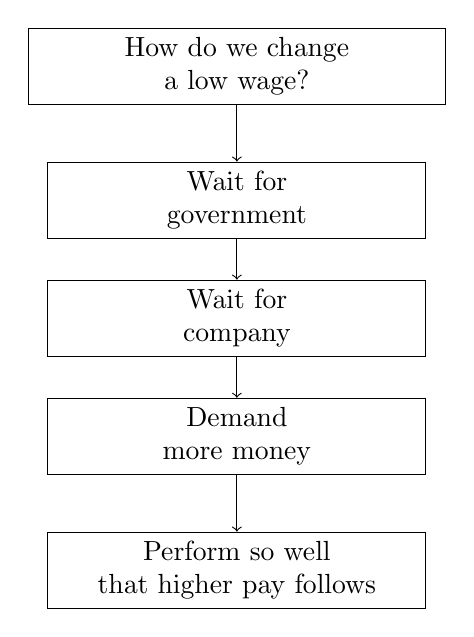
\begin{tikzpicture}[x=1cm,y=1cm]
\node[draw, rectangle, align=center, minimum width=5.3cm, minimum height=0.9cm] (top) at (0,0) {How do we change\\a low wage?};
\node[draw, rectangle, align=center, minimum width=4.8cm, minimum height=0.8cm] (g) at (0,-1.7) {Wait for\\government};
\node[draw, rectangle, align=center, minimum width=4.8cm, minimum height=0.8cm] (c) at (0,-3.2) {Wait for\\company};
\node[draw, rectangle, align=center, minimum width=4.8cm, minimum height=0.8cm] (d) at (0,-4.7) {Demand\\more money};
\node[draw, rectangle, align=center, minimum width=4.8cm, minimum height=0.9cm] (p) at (0,-6.4) {Perform so well\\that higher pay follows};
\draw[->] (top) -- (g);
\draw[->] (g) -- (c);
\draw[->] (c) -- (d);
\draw[->] (d) -- (p);
\end{tikzpicture}
\caption{A transcript-derived reconstruction of the lecture's opening sequence. Rohn moves through three weak strategies before keeping performance as the decisive philosophy.}
\end{figure}

What he keeps is the philosophy of performance. The worker does not merely wait for a new wage; the worker becomes the sort of worker for whom the old wage no longer fits. In this sense the lecture shifts very early from external pressure to internal development.

\subsection{Question \& Answer}

\paragraph{Question.} If demand can move a wage from \(5\) to \(6\), why is it still not the road to wealth?

\paragraph{Answer.} In the lecture's logic, demand acts on the employer from the outside, and only intermittently. Performance acts on the value of the worker from the inside, and can continue to scale. A group demand may secure a raise; it does not by itself explain how one climbs an entire economic ladder.

This is why the lecture now turns from small wage changes to a much larger question: what if we stop asking for a dollar more and ask instead whether income itself can be multiplied?

\section{The Income-Multiplication Ladder}

Having rejected the weaker strategies, Rohn makes the problem suddenly larger. If someone can be found at \( \$5 \) an hour and someone else at \( \$50 \) an hour, then the lecture wants us to face a simple but unsettling operation:
\begin{equation}
w \mapsto 10w.
\end{equation}
This is the first real mathematical spine of the talk. It is not formal economics. It is repeated arithmetic used to train the imagination.

The lecture then stacks the operation several times:
\begin{align}
w_0 &= \$5/\text{hour}, \\
w_1 &= 10w_0 = \$50/\text{hour}, \\
w_2 &= 10w_1 = \$500/\text{hour}, \\
w_3 &= 10w_2 = \$5{,}000/\text{hour}, \\
w_4 &= 10w_3 = \$50{,}000/\text{hour}.
\end{align}
Rohn does not present this as a law of nature. He presents it as a sequence of existence questions. Do we know anyone at the next rung? If yes, then the arithmetic obstacle is gone. What remains is the human obstacle.

The talk strengthens this sequence by using examples above the nominal ladder. General Schwarzkopf is said to receive about
\begin{equation}
w_{\mathrm{speech}} \approx \$65{,}000/\text{hour},
\end{equation}
which functions in the lecture as a social proof that the upper rungs are not imaginary.

\subsection{Question \& Answer}

\paragraph{Question.} If income can be multiplied by ten once, why not again, and again?

\paragraph{Answer.} The arithmetic itself offers no resistance. Once the operation \(w \mapsto 10w\) is accepted at one stage, the lecture uses the existence of people at the next stage to show that no conceptual barrier remains. The genuine problem is not numerical possibility but the transformation of the person who would occupy the higher rung.

The lecture therefore moves from arithmetic possibility to a rule of development. We have learned that the ladder may exist. We now have to ask how one climbs it.

\section{Working on Yourself and Becoming Attractive}

Rohn answers the question of ascent with a rule so compressed that it almost behaves like an update equation:
\begin{equation}
\text{job work} \to \text{living}, \qquad \text{self work} \to \text{fortune}.
\end{equation}
This is not written by the speaker as formal notation, but it faithfully compresses the distinction he insists on. If we work hard on the job, we may make a living. If we work hard on ourselves, we may make a fortune.

We can restate the lecture's mechanism in a more explicit chain:
\begin{equation}
\text{economic ascent} \Rightarrow \text{self-development} \Rightarrow \text{greater value to the marketplace}.
\end{equation}
That language prepares the next step, where success is no longer described as something chased directly. It is described as something attracted by the person we become.

\begin{definition}
In the language of this lecture, \emph{success as attraction} means that success is not first pursued as an external object. Rather, success follows from becoming a more attractive person to the marketplace.
\end{definition}

The importance of this move is structural. The lecture began with wages and has now reached anthropology. We are no longer asking only what pay scale exists; we are asking what kind of person can enter that scale.

At this point the lecture broadens again. The change is no longer merely private. Rohn wants to say that we live in a historical moment especially suited to such growth.

\section{The Twenty-First Century, Opportunity, and the Gift of Words}

The lecture now makes a larger claim: the early twenty-first century is a time of unusual opportunity, but also of unusual competition. This pairing matters. The talk does not offer pure optimism. It says, in effect, that the world is historically open, but that openness demands stronger internal equipment.

Rohn's compact historical formula may be written schematically as
\begin{equation}
\text{human history} \sim \text{opportunity} + \text{difficulty},
\end{equation}
and alongside it,
\begin{equation}
\text{human history} \sim \text{tyranny} + \text{liberty}.
\end{equation}
He also gives a few fixed numerical anchors, among them the claim that World War II cost about
\begin{equation}
50\,\text{million}
\end{equation}
lives, of which about
\begin{equation}
19\,\text{million}
\end{equation}
were Russian. These figures are not developed into formal argument, but they do provide scale for his claim that the century has turned into a different historical environment.

\subsection{Question \& Answer}

\paragraph{Question.} If this is a time of unprecedented opportunity, how do we actually use it?

\paragraph{Answer.} Rohn's answer is not first a policy or a business model. It is \emph{mind}, and then \emph{words}. The lecture treats words as an instrument that gives light, and therefore sight, and therefore direction.

This move can be written in a compact causal form:
\begin{equation}
\text{words} \to \text{light} \to \text{sight} \to \text{decision} \to \text{change}.
\end{equation}
What matters here is that language is not decorative. It is operational.

Rohn then decomposes communication into three parts:
\begin{enumerate}
\item \textbf{Training}: showing someone how to do the business or job.
\item \textbf{Teaching}: conveying life skills, leadership, management, and disciplined practice.
\item \textbf{Inspiring}: helping someone see himself better than he presently is, and helping him imagine a future self.
\end{enumerate}
In the lecture, this triad is already economic. Training pays. Teaching enlarges capability. Inspiring changes the scale of possibility.

The next transition is therefore natural. If words enlarge sight, what do we actually see when we look at life economically? Rohn answers with the language of fruitfulness and productivity.

\section{Fruitfulness, Productivity, and the Higher Life}

Rohn explicitly glosses ``be fruitful'' as ``be productive.'' That is an important translation, because it turns a moral or biblical phrase into an economic and practical one.

\begin{definition}
Within this lecture, \emph{fruitfulness} means productivity: the capacity to produce not only for immediate survival but for larger circles of responsibility.
\end{definition}

The lecture then builds a ladder of widening provision:
\begin{align}
\text{self} &\to \text{self + spouse} \to \text{self + family} \\
&\to \text{generosity} \to \text{large surplus for others}.
\end{align}
The sequence matters. Survival is not denied; it is treated as the first threshold. But survival alone is not yet the good life. Marriage requires more than solitary provision. Children require more again. Generosity requires more than family maintenance. The highest rungs involve large productive surplus.

\subsection{Question \& Answer}

\paragraph{Question.} Why should we produce more than we need for ourselves and our family?

\paragraph{Answer.} The lecture's answer is that a higher life opens only when provision exceeds immediate need. Surplus creates generosity, support for worthy projects, and eventually wealth creation for others. The issue is not indulgence but enlargement of responsibility.

Rohn gives a worked example:
\begin{align}
P &= \$10\,\text{million}, \\
N &= \$3\,\text{million}, \\
S &= P-N = \$7\,\text{million}.
\end{align}
Here \(P\) is yearly production, \(N\) is yearly family need, and \(S\) is surplus. The lecture's interpretation of \(S\) is not luxury consumption. It is giving capacity.

This same pattern appears in the Mark Hughes example. The numbers are presented as business imagination on a large scale:
\begin{align}
V_{\mathrm{company}} &\approx \$680\,\text{million}, \\
L_{\mathrm{son}} &\approx \$350\,\text{million}, \\
W_{\mathrm{others}} &\approx \$3.5\,\text{billion}.
\end{align}
Rohn's point is not to do valuation theory. His point is to show that economic life can be ordered so that wealth radiates outward rather than terminating in the producer.

Once he has enlarged the target this far, he deliberately narrows the lecture again and returns to basics.

\section{Fundamentals, Ratios, and the 80--20 Rule}

Rohn insists that fundamentals are few and old. This is a structural corrective to the earlier expansiveness. Once we have been shown extraordinary possibility, we are told not to look for exotic secrets. Truth is old. Fundamentals are few. Skill is antique, not newly manufactured.

The most formal arithmetic in this part of the lecture is the law of averages. The speaker states it verbally: if we do something often enough, we will soon have a ratio of results. Since no board equation survives, we use a cautious shorthand:
\begin{equation}
R=\frac{s}{n},
\end{equation}
where \(n\) is the number of attempts and \(s\) is the number of successful outcomes.

The lecture's example is simple:
\begin{align}
n&=10 \quad \Longrightarrow \quad s=1,\\
n&=10 \quad \Longrightarrow \quad s=2 \quad \text{after improved skill}.
\end{align}
The meaning is not that the law changes. The skill changes, and the ratio improves.

This leads into the better-known distribution rule:
\begin{equation}
20\%\text{ of the people do }80\%\text{ of the work},\qquad
80\%\text{ do }20\%.
\end{equation}
Rohn then draws a managerial corollary:
\begin{equation}
t_{20}=0.8T, \qquad t_{80}=0.2T,
\end{equation}
meaning that \(80\%\) of available time \(T\) should be spent with the productive \(20\%\), and only \(20\%\) with the remaining \(80\%\).

\subsection{Question \& Answer}

\paragraph{Question.} Why do different people react so differently to the same seminar or presentation?

\paragraph{Answer.} The lecture treats this not as an accident but as part of the law of averages itself. Some laugh, some mock, some do not understand, and some believe. The same message passes through a distribution rather than producing a uniform result. This is why the speaker treats ratios and percentages as practical knowledge rather than as pessimism.

The Peter example supplies a striking count:
\begin{equation}
\text{believers} \approx 3000.
\end{equation}
Again, the point is not exact statistics. It is that human response has a structure, and the speaker must learn to work within that structure.

Having returned to ratios and basics, the lecture is now ready to name the master term under which all of the earlier material is gathered: personal philosophy.

\section{Personal Philosophy, Danger and Opportunity, and the Return to Profits}

Rohn's largest claim is that each person's personal philosophy is the greatest determining factor in how life works out. This is where the lecture's opening word, \emph{philosophy}, returns with greater weight than before.

\begin{definition}
A \emph{personal philosophy}, in the operational sense used by this lecture, is a guidance system.
\end{definition}

That guidance system has two functions only:
\begin{equation}
\text{danger} \to \text{minimize}, \qquad \text{opportunity} \to \text{maximize}.
\end{equation}
We may summarize the point schematically as
\begin{equation}
\text{good life} \sim \min(\text{dangers})+\max(\text{opportunities}),
\end{equation}
with the understanding that this is a note-writer's shorthand, not the speaker's own formal notation.

\subsection{Question \& Answer}

\paragraph{Question.} Why is life both danger and opportunity?

\paragraph{Answer.} Here the lecture no longer offers arithmetic but a storyteller's explanation. Rohn proposes, cautiously and repeatedly, that it \emph{seems like} human life is framed as a great adventure. In that frame, danger is not a removable defect of existence; it is part of the structure within which opportunity becomes meaningful. The long theological material about Lucifer and Job is used not to prove a doctrine but to keep this tension intact.

Once this tension is named, the closing practical instructions make sense. We learn from what we see. We learn from what we hear. We learn from what we read. We guard the door of the mind. We choose inputs. We return to assemblies. We continue reading.

The learning channels may therefore be written compactly as
\begin{equation}
\text{sight}, \qquad \text{hearing}, \qquad \text{reading}.
\end{equation}
And the rule governing them is one of disciplined selection, not indiscriminate intake.

The lecture then closes by returning to the economic distinction from which it began. After all the widening motions of the talk, we come back to the compressed pair:
\begin{equation}
\text{wages} \to \text{living}, \qquad \text{profits} \to \text{fortune}.
\end{equation}
This return is structurally important. The lecture begins with wages, rises through multiplication, development, words, productivity, fundamentals, and philosophy, and then circles back to a simpler sentence that now carries the whole weight of the journey.

\section{Summary}

The chapter has followed the lecture's own progression: weak economic philosophies are tested and left behind; performance becomes the live option; a repeated tenfold map of income trains the imagination; self-development becomes the mechanism of ascent; success is recast as attraction; the century is described as open but competitive; words become an economic instrument; fruitfulness becomes productivity; surplus becomes generosity; ratios and the 80--20 rule return us to fundamentals; and personal philosophy is finally defined as a guidance system for danger and opportunity.

The lecture's closing compression is worth keeping in view. We do not merely ask for more. We become more. And once that change is admitted, the arithmetic ladder, the productivity ladder, and the guidance system all become parts of a single argument about how a life may be deliberately enlarged.